% Options for packages loaded elsewhere
\PassOptionsToPackage{unicode}{hyperref}
\PassOptionsToPackage{hyphens}{url}
%
\documentclass[
]{article}
\usepackage{amsmath,amssymb}
\usepackage{iftex}
\ifPDFTeX
  \usepackage[T1]{fontenc}
  \usepackage[utf8]{inputenc}
  \usepackage{textcomp} % provide euro and other symbols
\else % if luatex or xetex
  \usepackage{unicode-math} % this also loads fontspec
  \defaultfontfeatures{Scale=MatchLowercase}
  \defaultfontfeatures[\rmfamily]{Ligatures=TeX,Scale=1}
\fi
\usepackage{lmodern}
\ifPDFTeX\else
  % xetex/luatex font selection
\fi
% Use upquote if available, for straight quotes in verbatim environments
\IfFileExists{upquote.sty}{\usepackage{upquote}}{}
\IfFileExists{microtype.sty}{% use microtype if available
  \usepackage[]{microtype}
  \UseMicrotypeSet[protrusion]{basicmath} % disable protrusion for tt fonts
}{}
\makeatletter
\@ifundefined{KOMAClassName}{% if non-KOMA class
  \IfFileExists{parskip.sty}{%
    \usepackage{parskip}
  }{% else
    \setlength{\parindent}{0pt}
    \setlength{\parskip}{6pt plus 2pt minus 1pt}}
}{% if KOMA class
  \KOMAoptions{parskip=half}}
\makeatother
\usepackage{xcolor}
\usepackage[margin=1in]{geometry}
\usepackage{color}
\usepackage{fancyvrb}
\newcommand{\VerbBar}{|}
\newcommand{\VERB}{\Verb[commandchars=\\\{\}]}
\DefineVerbatimEnvironment{Highlighting}{Verbatim}{commandchars=\\\{\}}
% Add ',fontsize=\small' for more characters per line
\usepackage{framed}
\definecolor{shadecolor}{RGB}{248,248,248}
\newenvironment{Shaded}{\begin{snugshade}}{\end{snugshade}}
\newcommand{\AlertTok}[1]{\textcolor[rgb]{0.94,0.16,0.16}{#1}}
\newcommand{\AnnotationTok}[1]{\textcolor[rgb]{0.56,0.35,0.01}{\textbf{\textit{#1}}}}
\newcommand{\AttributeTok}[1]{\textcolor[rgb]{0.13,0.29,0.53}{#1}}
\newcommand{\BaseNTok}[1]{\textcolor[rgb]{0.00,0.00,0.81}{#1}}
\newcommand{\BuiltInTok}[1]{#1}
\newcommand{\CharTok}[1]{\textcolor[rgb]{0.31,0.60,0.02}{#1}}
\newcommand{\CommentTok}[1]{\textcolor[rgb]{0.56,0.35,0.01}{\textit{#1}}}
\newcommand{\CommentVarTok}[1]{\textcolor[rgb]{0.56,0.35,0.01}{\textbf{\textit{#1}}}}
\newcommand{\ConstantTok}[1]{\textcolor[rgb]{0.56,0.35,0.01}{#1}}
\newcommand{\ControlFlowTok}[1]{\textcolor[rgb]{0.13,0.29,0.53}{\textbf{#1}}}
\newcommand{\DataTypeTok}[1]{\textcolor[rgb]{0.13,0.29,0.53}{#1}}
\newcommand{\DecValTok}[1]{\textcolor[rgb]{0.00,0.00,0.81}{#1}}
\newcommand{\DocumentationTok}[1]{\textcolor[rgb]{0.56,0.35,0.01}{\textbf{\textit{#1}}}}
\newcommand{\ErrorTok}[1]{\textcolor[rgb]{0.64,0.00,0.00}{\textbf{#1}}}
\newcommand{\ExtensionTok}[1]{#1}
\newcommand{\FloatTok}[1]{\textcolor[rgb]{0.00,0.00,0.81}{#1}}
\newcommand{\FunctionTok}[1]{\textcolor[rgb]{0.13,0.29,0.53}{\textbf{#1}}}
\newcommand{\ImportTok}[1]{#1}
\newcommand{\InformationTok}[1]{\textcolor[rgb]{0.56,0.35,0.01}{\textbf{\textit{#1}}}}
\newcommand{\KeywordTok}[1]{\textcolor[rgb]{0.13,0.29,0.53}{\textbf{#1}}}
\newcommand{\NormalTok}[1]{#1}
\newcommand{\OperatorTok}[1]{\textcolor[rgb]{0.81,0.36,0.00}{\textbf{#1}}}
\newcommand{\OtherTok}[1]{\textcolor[rgb]{0.56,0.35,0.01}{#1}}
\newcommand{\PreprocessorTok}[1]{\textcolor[rgb]{0.56,0.35,0.01}{\textit{#1}}}
\newcommand{\RegionMarkerTok}[1]{#1}
\newcommand{\SpecialCharTok}[1]{\textcolor[rgb]{0.81,0.36,0.00}{\textbf{#1}}}
\newcommand{\SpecialStringTok}[1]{\textcolor[rgb]{0.31,0.60,0.02}{#1}}
\newcommand{\StringTok}[1]{\textcolor[rgb]{0.31,0.60,0.02}{#1}}
\newcommand{\VariableTok}[1]{\textcolor[rgb]{0.00,0.00,0.00}{#1}}
\newcommand{\VerbatimStringTok}[1]{\textcolor[rgb]{0.31,0.60,0.02}{#1}}
\newcommand{\WarningTok}[1]{\textcolor[rgb]{0.56,0.35,0.01}{\textbf{\textit{#1}}}}
\usepackage{graphicx}
\makeatletter
\newsavebox\pandoc@box
\newcommand*\pandocbounded[1]{% scales image to fit in text height/width
  \sbox\pandoc@box{#1}%
  \Gscale@div\@tempa{\textheight}{\dimexpr\ht\pandoc@box+\dp\pandoc@box\relax}%
  \Gscale@div\@tempb{\linewidth}{\wd\pandoc@box}%
  \ifdim\@tempb\p@<\@tempa\p@\let\@tempa\@tempb\fi% select the smaller of both
  \ifdim\@tempa\p@<\p@\scalebox{\@tempa}{\usebox\pandoc@box}%
  \else\usebox{\pandoc@box}%
  \fi%
}
% Set default figure placement to htbp
\def\fps@figure{htbp}
\makeatother
\setlength{\emergencystretch}{3em} % prevent overfull lines
\providecommand{\tightlist}{%
  \setlength{\itemsep}{0pt}\setlength{\parskip}{0pt}}
\setcounter{secnumdepth}{-\maxdimen} % remove section numbering
\usepackage{booktabs}
\usepackage{longtable}
\usepackage{array}
\usepackage{multirow}
\usepackage{wrapfig}
\usepackage{float}
\usepackage{colortbl}
\usepackage{pdflscape}
\usepackage{tabu}
\usepackage{threeparttable}
\usepackage{threeparttablex}
\usepackage[normalem]{ulem}
\usepackage{makecell}
\usepackage{xcolor}
\usepackage{bookmark}
\IfFileExists{xurl.sty}{\usepackage{xurl}}{} % add URL line breaks if available
\urlstyle{same}
\hypersetup{
  pdftitle={Check genotype data using PLINK QC reports},
  pdfauthor={Haesu Ko},
  hidelinks,
  pdfcreator={LaTeX via pandoc}}

\title{Check genotype data using PLINK QC reports}
\author{Haesu Ko}
\date{2025-08-21}

\begin{document}
\maketitle

\subsection{Overview}\label{overview}

{ℹ️} Quick checks of PLINK2 QC reports (.smiss, .vmiss, .hardy, .afreq)
per breed:

Load PLINK2 QC report files

Preview them

Plot missingness, HWE, and MAF per breed

Write CSVs of outliers and a combined summary for failing SNPs

📁 PLINK2 QC reports at a glance

.smiss --- sample missingness

Per-individual missing call rate (F\_MISS by sample).

.vmiss --- variant missingness

Per-variant missing call rate across samples (F\_MISS by SNP).

.hardy / .hardy.x --- HWE

Hardy--Weinberg exact test P-values (autosomes / chrX).

.afreq --- allele frequency

Per-variant alternate (ALT) allele frequency (uses the alleles from the
.pvar; ALT here is not forced to be minor, so frequencies can be
\textgreater{} 0.5.).

\paragraph{PLINK2 commands used to generate these outputs per
breed}\label{plink2-commands-used-to-generate-these-outputs-per-breed}

{🐄} Holstein

Expected output files:
02\_reports/holstein/NIAS\_ibv3\_296ea.holstein.autosomesX.{[}smiss\textbar vmiss\textbar hardy\textbar afreq{]}

{🧀} Jersey

Expected output files:
02\_reports/jersey/NIAS\_ibv3\_296ea.jersey.autosomesX.{[}smiss\textbar vmiss\textbar hardy\textbar afreq{]}

{⚙️} PLINK2 arguments used

-\/-pfile PREFIX

Load PGEN dataset (PREFIX.pgen/pvar/psam).

-\/-missing

Calculate missing call rates (writes .smiss \& .vmiss).

-\/-hardy

Run Hardy--Weinberg exact test (autosomes → .hardy, chrX → .hardy.x).

-\/-freq

Compute allele frequencies (writes .afreq).

-\/-out PREFIX

Set output prefix/path; directory must exist.

\subsection{Setup}\label{setup}

\begin{Shaded}
\begin{Highlighting}[]
\CommentTok{\# Basic QC reports for each breed}
\CommentTok{\# {-}{-}{-}{-}{-}{-}{-}{-}{-}{-}{-}{-}{-}{-}{-}{-}{-}{-}{-}{-}{-}{-}{-}{-}{-}{-}{-}{-}{-}{-}{-}{-}{-}{-}{-}{-}{-}{-}{-}{-}{-}{-}{-}{-}{-}{-}{-}{-}{-}{-}{-}}
\CommentTok{\# {-}{-}{-}{-} packages {-}{-}{-}{-}}
\NormalTok{need }\OtherTok{\textless{}{-}} \FunctionTok{c}\NormalTok{(}\StringTok{"readr"}\NormalTok{,}\StringTok{"dplyr"}\NormalTok{,}\StringTok{"ggplot2"}\NormalTok{)}
\NormalTok{to\_install }\OtherTok{\textless{}{-}} \FunctionTok{setdiff}\NormalTok{(need, }\FunctionTok{rownames}\NormalTok{(}\FunctionTok{installed.packages}\NormalTok{()))}
\ControlFlowTok{if}\NormalTok{ (}\FunctionTok{length}\NormalTok{(to\_install)) }\FunctionTok{install.packages}\NormalTok{(to\_install, }\AttributeTok{repos =} \StringTok{"https://cloud.r{-}project.org"}\NormalTok{)}
\FunctionTok{invisible}\NormalTok{(}\FunctionTok{lapply}\NormalTok{(need, library, }\AttributeTok{character.only =} \ConstantTok{TRUE}\NormalTok{))}

\CommentTok{\# {-}{-}{-}{-} helpers \& thresholds {-}{-}{-}{-}}
\NormalTok{neglog10 }\OtherTok{\textless{}{-}} \ControlFlowTok{function}\NormalTok{(p) }\SpecialCharTok{{-}}\FunctionTok{log10}\NormalTok{(}\FunctionTok{pmax}\NormalTok{(p, .Machine}\SpecialCharTok{$}\NormalTok{double.xmin))  }\CommentTok{\# avoid {-}Inf}

\CommentTok{\# MAF for biallelic data: use ALT\_FREQS}
\CommentTok{\# ALT in plink2 {-}{-}freq reflects non{-}reference (VCF/PVAR) by default; it is not guaranteed to be the minor allele.}

\NormalTok{maf\_from\_afreq }\OtherTok{\textless{}{-}} \ControlFlowTok{function}\NormalTok{(df) \{}
  \FunctionTok{stopifnot}\NormalTok{(}\StringTok{"ALT\_FREQS"} \SpecialCharTok{\%in\%} \FunctionTok{names}\NormalTok{(df))}
\NormalTok{  df }\SpecialCharTok{\%\textgreater{}\%}
    \FunctionTok{mutate}\NormalTok{(}
      \CommentTok{\# ensure numeric and clamp to [0,1] just in case}
      \AttributeTok{ALT\_FREQS =} \FunctionTok{suppressWarnings}\NormalTok{(}\FunctionTok{as.numeric}\NormalTok{(ALT\_FREQS)),}
      \AttributeTok{ALT\_FREQS =} \FunctionTok{pmin}\NormalTok{(}\FunctionTok{pmax}\NormalTok{(ALT\_FREQS, }\DecValTok{0}\NormalTok{), }\DecValTok{1}\NormalTok{),}
      \AttributeTok{MAF\_calc  =} \FunctionTok{pmin}\NormalTok{(ALT\_FREQS, }\DecValTok{1} \SpecialCharTok{{-}}\NormalTok{ ALT\_FREQS)}
\NormalTok{    )}
\NormalTok{\}}

\CommentTok{\# {-}{-}{-}{-} thresholds (tune to taste) {-}{-}{-}{-}}
\NormalTok{mind\_thr }\OtherTok{\textless{}{-}} \FloatTok{0.05}  \CommentTok{\# per{-}sample missingness}
\NormalTok{geno\_thr }\OtherTok{\textless{}{-}} \FloatTok{0.05}  \CommentTok{\# per{-}variant missingness}
\NormalTok{hwe\_thr  }\OtherTok{\textless{}{-}} \FloatTok{1e{-}6}  \CommentTok{\# HWE p{-}value}
\NormalTok{maf\_thr  }\OtherTok{\textless{}{-}} \FloatTok{0.05}  \CommentTok{\# MAF}

\CommentTok{\# {-}{-}{-}{-} base path \& breeds {-}{-}{-}{-}}
\NormalTok{base\_dir }\OtherTok{\textless{}{-}} \StringTok{"02\_reports"}
\NormalTok{breeds   }\OtherTok{\textless{}{-}} \FunctionTok{c}\NormalTok{(}\StringTok{"holstein"}\NormalTok{,}\StringTok{"jersey"}\NormalTok{)}
\end{Highlighting}
\end{Shaded}

🔧 Run parameters

Base directory (base\_dir)

02\_reports

Breeds (breeds)

holstein, jersey

Per-sample missingness (mind\_thr)

0.05

Per-variant missingness (geno\_thr)

0.05

HWE p-value threshold (hwe\_thr)

1e-06

MAF threshold (maf\_thr)

0.05

\subsection{Per-breed checks}\label{per-breed-checks}

\begin{Shaded}
\begin{Highlighting}[]
\CommentTok{\# collect per{-}breed summary rows here}
\NormalTok{summary\_rows }\OtherTok{\textless{}{-}} \FunctionTok{list}\NormalTok{()}

\CommentTok{\# {-}{-}{-}{-} Run for each breed {-}{-}{-}{-}}
\CommentTok{\# For holstein}
\NormalTok{breed }\OtherTok{=}\NormalTok{ breeds[}\DecValTok{1}\NormalTok{]}
\CommentTok{\# For jersey}
\NormalTok{breed }\OtherTok{=}\NormalTok{ breeds[}\DecValTok{2}\NormalTok{]}

\CommentTok{\# {-}{-}{-}{-} Automatic run across breeds {-}{-}{-}{-}}
\ControlFlowTok{for}\NormalTok{ (breed }\ControlFlowTok{in}\NormalTok{ breeds) \{}
  \FunctionTok{message}\NormalTok{(}\StringTok{"=== Processing breed: "}\NormalTok{, breed, }\StringTok{" ==="}\NormalTok{)}
  
  \CommentTok{\# Matches your plink2 {-}{-}out prefixes:}
  \CommentTok{\#   02\_reports/holstein/NIAS\_ibv3\_296ea.holstein.autosomesX}
  \CommentTok{\#   02\_reports/jersey/NIAS\_ibv3\_296ea.jersey.autosomesX}
\NormalTok{  prefix }\OtherTok{\textless{}{-}} \FunctionTok{file.path}\NormalTok{(base\_dir, breed, }\FunctionTok{sprintf}\NormalTok{(}\StringTok{"NIAS\_ibv3\_296ea.\%s.autosomesX"}\NormalTok{, breed))}
  
\NormalTok{  f\_smiss }\OtherTok{\textless{}{-}} \FunctionTok{paste0}\NormalTok{(prefix, }\StringTok{".smiss"}\NormalTok{)}
\NormalTok{  f\_vmiss }\OtherTok{\textless{}{-}} \FunctionTok{paste0}\NormalTok{(prefix, }\StringTok{".vmiss"}\NormalTok{)}
\NormalTok{  f\_hardy }\OtherTok{\textless{}{-}} \FunctionTok{paste0}\NormalTok{(prefix, }\StringTok{".hardy"}\NormalTok{)}
\NormalTok{  f\_afreq }\OtherTok{\textless{}{-}} \FunctionTok{paste0}\NormalTok{(prefix, }\StringTok{".afreq"}\NormalTok{)}
  
\NormalTok{  out\_dir  }\OtherTok{\textless{}{-}} \FunctionTok{file.path}\NormalTok{(base\_dir, breed)}
\NormalTok{  figs\_dir }\OtherTok{\textless{}{-}} \FunctionTok{file.path}\NormalTok{(out\_dir, }\StringTok{"figs"}\NormalTok{)}
  \FunctionTok{dir.create}\NormalTok{(figs\_dir, }\AttributeTok{showWarnings =} \ConstantTok{FALSE}\NormalTok{, }\AttributeTok{recursive =} \ConstantTok{TRUE}\NormalTok{)}
  
  \CommentTok{\# {-}{-}{-}{-} load {-}{-}{-}{-}}
\NormalTok{  smiss }\OtherTok{\textless{}{-}}\NormalTok{ readr}\SpecialCharTok{::}\FunctionTok{read\_tsv}\NormalTok{(f\_smiss, }\AttributeTok{show\_col\_types =} \ConstantTok{FALSE}\NormalTok{) }\SpecialCharTok{\%\textgreater{}\%}
\NormalTok{    dplyr}\SpecialCharTok{::}\FunctionTok{rename}\NormalTok{(}\AttributeTok{FID =} \StringTok{\textasciigrave{}}\AttributeTok{\#FID}\StringTok{\textasciigrave{}}\NormalTok{)  }\CommentTok{\# "\#FID" {-}\textgreater{} FID}
  
\NormalTok{  vmiss }\OtherTok{\textless{}{-}}\NormalTok{ readr}\SpecialCharTok{::}\FunctionTok{read\_tsv}\NormalTok{(f\_vmiss, }\AttributeTok{show\_col\_types =} \ConstantTok{FALSE}\NormalTok{) }\SpecialCharTok{\%\textgreater{}\%}
\NormalTok{    dplyr}\SpecialCharTok{::}\FunctionTok{rename}\NormalTok{(}\AttributeTok{CHROM =} \StringTok{\textasciigrave{}}\AttributeTok{\#CHROM}\StringTok{\textasciigrave{}}\NormalTok{)}
  
\NormalTok{  hardy }\OtherTok{\textless{}{-}}\NormalTok{ readr}\SpecialCharTok{::}\FunctionTok{read\_tsv}\NormalTok{(f\_hardy, }\AttributeTok{show\_col\_types =} \ConstantTok{FALSE}\NormalTok{) }\SpecialCharTok{\%\textgreater{}\%}
\NormalTok{    dplyr}\SpecialCharTok{::}\FunctionTok{rename}\NormalTok{(}\AttributeTok{CHROM =} \StringTok{\textasciigrave{}}\AttributeTok{\#CHROM}\StringTok{\textasciigrave{}}\NormalTok{) }\SpecialCharTok{\%\textgreater{}\%}
    \FunctionTok{mutate}\NormalTok{(}\AttributeTok{minuslog10P =} \FunctionTok{neglog10}\NormalTok{(P))}
  
\NormalTok{  afreq }\OtherTok{\textless{}{-}}\NormalTok{ readr}\SpecialCharTok{::}\FunctionTok{read\_tsv}\NormalTok{(f\_afreq, }\AttributeTok{show\_col\_types =} \ConstantTok{FALSE}\NormalTok{) }\SpecialCharTok{\%\textgreater{}\%}
\NormalTok{    dplyr}\SpecialCharTok{::}\FunctionTok{rename}\NormalTok{(}\AttributeTok{CHROM =} \StringTok{\textasciigrave{}}\AttributeTok{\#CHROM}\StringTok{\textasciigrave{}}\NormalTok{) }\SpecialCharTok{\%\textgreater{}\%}
    \FunctionTok{maf\_from\_afreq}\NormalTok{()}
  
  \CommentTok{\# Peek}
  \FunctionTok{message}\NormalTok{(}\StringTok{"smiss head:"}\NormalTok{); }\FunctionTok{print}\NormalTok{(utils}\SpecialCharTok{::}\FunctionTok{head}\NormalTok{(smiss))}
  \FunctionTok{message}\NormalTok{(}\StringTok{"vmiss head:"}\NormalTok{); }\FunctionTok{print}\NormalTok{(utils}\SpecialCharTok{::}\FunctionTok{head}\NormalTok{(vmiss))}
  \FunctionTok{message}\NormalTok{(}\StringTok{"hardy head:"}\NormalTok{); }\FunctionTok{print}\NormalTok{(utils}\SpecialCharTok{::}\FunctionTok{head}\NormalTok{(hardy))}
  \FunctionTok{message}\NormalTok{(}\StringTok{"afreq head:"}\NormalTok{); }\FunctionTok{print}\NormalTok{(utils}\SpecialCharTok{::}\FunctionTok{head}\NormalTok{(afreq))}
  
  \CommentTok{\# {-}{-}{-}{-} plots {-}{-}{-}{-}}
\NormalTok{  p1 }\OtherTok{\textless{}{-}} \FunctionTok{ggplot}\NormalTok{(smiss, }\FunctionTok{aes}\NormalTok{(}\AttributeTok{x =}\NormalTok{ F\_MISS)) }\SpecialCharTok{+}
    \FunctionTok{geom\_histogram}\NormalTok{(}\AttributeTok{bins =} \DecValTok{50}\NormalTok{) }\SpecialCharTok{+}
    \FunctionTok{geom\_vline}\NormalTok{(}\AttributeTok{xintercept =}\NormalTok{ mind\_thr) }\SpecialCharTok{+}
    \FunctionTok{labs}\NormalTok{(}\AttributeTok{title =} \FunctionTok{paste0}\NormalTok{(breed, }\StringTok{": sample missingness (F\_MISS)"}\NormalTok{),}
         \AttributeTok{x =} \StringTok{"F\_MISS"}\NormalTok{, }\AttributeTok{y =} \StringTok{"Count"}\NormalTok{)}
  
\NormalTok{  p2 }\OtherTok{\textless{}{-}} \FunctionTok{ggplot}\NormalTok{(vmiss, }\FunctionTok{aes}\NormalTok{(}\AttributeTok{x =}\NormalTok{ F\_MISS)) }\SpecialCharTok{+}
    \FunctionTok{geom\_histogram}\NormalTok{(}\AttributeTok{bins =} \DecValTok{60}\NormalTok{) }\SpecialCharTok{+}
    \FunctionTok{geom\_vline}\NormalTok{(}\AttributeTok{xintercept =}\NormalTok{ geno\_thr) }\SpecialCharTok{+}
    \FunctionTok{labs}\NormalTok{(}\AttributeTok{title =} \FunctionTok{paste0}\NormalTok{(breed, }\StringTok{": variant missingness (F\_MISS)"}\NormalTok{),}
         \AttributeTok{x =} \StringTok{"F\_MISS"}\NormalTok{, }\AttributeTok{y =} \StringTok{"Count"}\NormalTok{)}
  
\NormalTok{  p3 }\OtherTok{\textless{}{-}} \FunctionTok{ggplot}\NormalTok{(hardy, }\FunctionTok{aes}\NormalTok{(}\AttributeTok{x =}\NormalTok{ minuslog10P)) }\SpecialCharTok{+}
    \FunctionTok{geom\_histogram}\NormalTok{(}\AttributeTok{bins =} \DecValTok{60}\NormalTok{) }\SpecialCharTok{+}
    \FunctionTok{geom\_vline}\NormalTok{(}\AttributeTok{xintercept =} \SpecialCharTok{{-}}\FunctionTok{log10}\NormalTok{(hwe\_thr)) }\SpecialCharTok{+}
    \FunctionTok{labs}\NormalTok{(}\AttributeTok{title =} \FunctionTok{paste0}\NormalTok{(breed, }\StringTok{": HWE ({-}log10P)"}\NormalTok{),}
         \AttributeTok{x =} \StringTok{"{-}log10(P)"}\NormalTok{, }\AttributeTok{y =} \StringTok{"Count"}\NormalTok{)}
  
\NormalTok{  p4 }\OtherTok{\textless{}{-}} \FunctionTok{ggplot}\NormalTok{(afreq, }\FunctionTok{aes}\NormalTok{(}\AttributeTok{x =}\NormalTok{ MAF\_calc)) }\SpecialCharTok{+}
    \FunctionTok{geom\_histogram}\NormalTok{(}\AttributeTok{bins =} \DecValTok{60}\NormalTok{) }\SpecialCharTok{+}
    \FunctionTok{geom\_vline}\NormalTok{(}\AttributeTok{xintercept =}\NormalTok{ maf\_thr) }\SpecialCharTok{+}
    \FunctionTok{labs}\NormalTok{(}\AttributeTok{title =} \FunctionTok{paste0}\NormalTok{(breed, }\StringTok{": MAF distribution"}\NormalTok{),}
         \AttributeTok{x =} \StringTok{"MAF"}\NormalTok{, }\AttributeTok{y =} \StringTok{"Count"}\NormalTok{)}
  
  \FunctionTok{print}\NormalTok{(p1); }\FunctionTok{print}\NormalTok{(p2); }\FunctionTok{print}\NormalTok{(p3); }\FunctionTok{print}\NormalTok{(p4)}
  
  \FunctionTok{ggsave}\NormalTok{(}\FunctionTok{file.path}\NormalTok{(figs\_dir, }\StringTok{"smiss\_hist.png"}\NormalTok{), p1, }\AttributeTok{width =} \DecValTok{3}\NormalTok{, }\AttributeTok{height =} \DecValTok{3}\NormalTok{, }\AttributeTok{dpi =} \DecValTok{300}\NormalTok{)}
  \FunctionTok{ggsave}\NormalTok{(}\FunctionTok{file.path}\NormalTok{(figs\_dir, }\StringTok{"vmiss\_hist.png"}\NormalTok{), p2, }\AttributeTok{width =} \DecValTok{3}\NormalTok{, }\AttributeTok{height =} \DecValTok{3}\NormalTok{, }\AttributeTok{dpi =} \DecValTok{300}\NormalTok{)}
  \FunctionTok{ggsave}\NormalTok{(}\FunctionTok{file.path}\NormalTok{(figs\_dir, }\StringTok{"hardy\_hist.png"}\NormalTok{), p3, }\AttributeTok{width =} \DecValTok{3}\NormalTok{, }\AttributeTok{height =} \DecValTok{3}\NormalTok{, }\AttributeTok{dpi =} \DecValTok{300}\NormalTok{)}
  \FunctionTok{ggsave}\NormalTok{(}\FunctionTok{file.path}\NormalTok{(figs\_dir, }\StringTok{"maf\_hist.png"}\NormalTok{),   p4, }\AttributeTok{width =} \DecValTok{3}\NormalTok{, }\AttributeTok{height =} \DecValTok{3}\NormalTok{, }\AttributeTok{dpi =} \DecValTok{300}\NormalTok{)}
  
  \CommentTok{\# {-}{-}{-}{-} outlier tables (breed{-}suffixed objects) {-}{-}{-}{-}}
  \FunctionTok{assign}\NormalTok{(}\FunctionTok{paste0}\NormalTok{(}\StringTok{"bad\_samples\_"}\NormalTok{,   breed),}
\NormalTok{         smiss }\SpecialCharTok{\%\textgreater{}\%} \FunctionTok{filter}\NormalTok{(F\_MISS }\SpecialCharTok{\textgreater{}}\NormalTok{ mind\_thr) }\SpecialCharTok{\%\textgreater{}\%} \FunctionTok{select}\NormalTok{(FID, IID, F\_MISS),}
         \AttributeTok{envir =}\NormalTok{ .GlobalEnv)}
  
  \FunctionTok{assign}\NormalTok{(}\FunctionTok{paste0}\NormalTok{(}\StringTok{"bad\_snps\_miss\_"}\NormalTok{, breed),}
\NormalTok{         vmiss }\SpecialCharTok{\%\textgreater{}\%} \FunctionTok{filter}\NormalTok{(F\_MISS }\SpecialCharTok{\textgreater{}}\NormalTok{ geno\_thr) }\SpecialCharTok{\%\textgreater{}\%} \FunctionTok{select}\NormalTok{(CHROM, ID, F\_MISS),}
         \AttributeTok{envir =}\NormalTok{ .GlobalEnv)}
  
  \FunctionTok{assign}\NormalTok{(}\FunctionTok{paste0}\NormalTok{(}\StringTok{"bad\_snps\_hwe\_"}\NormalTok{,  breed),}
\NormalTok{         hardy }\SpecialCharTok{\%\textgreater{}\%} \FunctionTok{filter}\NormalTok{(P }\SpecialCharTok{\textless{}}\NormalTok{ hwe\_thr) }\SpecialCharTok{\%\textgreater{}\%} \FunctionTok{select}\NormalTok{(CHROM, ID, P),}
         \AttributeTok{envir =}\NormalTok{ .GlobalEnv)}
  
  \FunctionTok{assign}\NormalTok{(}\FunctionTok{paste0}\NormalTok{(}\StringTok{"bad\_snps\_maf\_"}\NormalTok{,  breed),}
\NormalTok{         afreq }\SpecialCharTok{\%\textgreater{}\%} \FunctionTok{filter}\NormalTok{(MAF\_calc }\SpecialCharTok{\textless{}}\NormalTok{ maf\_thr) }\SpecialCharTok{\%\textgreater{}\%} \FunctionTok{select}\NormalTok{(CHROM, ID, MAF\_calc),}
         \AttributeTok{envir =}\NormalTok{ .GlobalEnv)}
  
  \CommentTok{\# (optional) if you want filenames to include the breed too, even though}
  \CommentTok{\# they already live in per{-}breed folders:}
\NormalTok{  readr}\SpecialCharTok{::}\FunctionTok{write\_csv}\NormalTok{(}\FunctionTok{get}\NormalTok{(}\FunctionTok{paste0}\NormalTok{(}\StringTok{"bad\_samples\_"}\NormalTok{,   breed)), }\FunctionTok{file.path}\NormalTok{(out\_dir, }\FunctionTok{paste0}\NormalTok{(}\StringTok{"bad\_samples\_over\_mind."}\NormalTok{, breed, }\StringTok{".csv"}\NormalTok{)))}
\NormalTok{  readr}\SpecialCharTok{::}\FunctionTok{write\_csv}\NormalTok{(}\FunctionTok{get}\NormalTok{(}\FunctionTok{paste0}\NormalTok{(}\StringTok{"bad\_snps\_miss\_"}\NormalTok{, breed)), }\FunctionTok{file.path}\NormalTok{(out\_dir, }\FunctionTok{paste0}\NormalTok{(}\StringTok{"bad\_snps\_over\_geno."}\NormalTok{, breed, }\StringTok{".csv"}\NormalTok{)))}
\NormalTok{  readr}\SpecialCharTok{::}\FunctionTok{write\_csv}\NormalTok{(}\FunctionTok{get}\NormalTok{(}\FunctionTok{paste0}\NormalTok{(}\StringTok{"bad\_snps\_hwe\_"}\NormalTok{,  breed)), }\FunctionTok{file.path}\NormalTok{(out\_dir, }\FunctionTok{paste0}\NormalTok{(}\StringTok{"bad\_snps\_hwe."}\NormalTok{, breed, }\StringTok{".csv"}\NormalTok{)))}
\NormalTok{  readr}\SpecialCharTok{::}\FunctionTok{write\_csv}\NormalTok{(}\FunctionTok{get}\NormalTok{(}\FunctionTok{paste0}\NormalTok{(}\StringTok{"bad\_snps\_maf\_"}\NormalTok{,  breed)), }\FunctionTok{file.path}\NormalTok{(out\_dir, }\FunctionTok{paste0}\NormalTok{(}\StringTok{"bad\_snps\_low\_maf."}\NormalTok{, breed, }\StringTok{".csv"}\NormalTok{)))}
  
  
  \CommentTok{\# {-}{-}{-}{-} combined per{-}variant table {-}{-}{-}{-}}
\NormalTok{  vmiss }\OtherTok{\textless{}{-}}\NormalTok{ vmiss }\SpecialCharTok{\%\textgreater{}\%} \FunctionTok{mutate}\NormalTok{(}\AttributeTok{CHROM =} \FunctionTok{as.character}\NormalTok{(CHROM))}
\NormalTok{  hardy }\OtherTok{\textless{}{-}}\NormalTok{ hardy }\SpecialCharTok{\%\textgreater{}\%} \FunctionTok{mutate}\NormalTok{(}\AttributeTok{CHROM =} \FunctionTok{as.character}\NormalTok{(CHROM))}
\NormalTok{  afreq }\OtherTok{\textless{}{-}}\NormalTok{ afreq }\SpecialCharTok{\%\textgreater{}\%} \FunctionTok{mutate}\NormalTok{(}\AttributeTok{CHROM =} \FunctionTok{as.character}\NormalTok{(CHROM))}
  
\NormalTok{  variant\_qc }\OtherTok{\textless{}{-}}\NormalTok{ vmiss }\SpecialCharTok{\%\textgreater{}\%}
    \FunctionTok{select}\NormalTok{(CHROM, ID, F\_MISS) }\SpecialCharTok{\%\textgreater{}\%}
    \FunctionTok{left\_join}\NormalTok{(}\FunctionTok{select}\NormalTok{(hardy, CHROM, ID, P),        }\AttributeTok{by =} \FunctionTok{c}\NormalTok{(}\StringTok{"CHROM"}\NormalTok{,}\StringTok{"ID"}\NormalTok{)) }\SpecialCharTok{\%\textgreater{}\%}
    \FunctionTok{left\_join}\NormalTok{(}\FunctionTok{select}\NormalTok{(afreq, CHROM, ID, MAF\_calc), }\AttributeTok{by =} \FunctionTok{c}\NormalTok{(}\StringTok{"CHROM"}\NormalTok{,}\StringTok{"ID"}\NormalTok{)) }\SpecialCharTok{\%\textgreater{}\%}
    \FunctionTok{mutate}\NormalTok{(}
      \AttributeTok{fail\_miss =}\NormalTok{ F\_MISS }\SpecialCharTok{\textgreater{}}\NormalTok{ geno\_thr,}
      \AttributeTok{fail\_hwe  =}\NormalTok{ P }\SpecialCharTok{\textless{}}\NormalTok{ hwe\_thr,}
      \AttributeTok{fail\_maf  =}\NormalTok{ MAF\_calc }\SpecialCharTok{\textless{}}\NormalTok{ maf\_thr,}
      \AttributeTok{fail\_any  =}\NormalTok{ fail\_miss }\SpecialCharTok{|}\NormalTok{ fail\_hwe }\SpecialCharTok{|}\NormalTok{ fail\_maf}
\NormalTok{    )}
  
\NormalTok{  readr}\SpecialCharTok{::}\FunctionTok{write\_csv}\NormalTok{(variant\_qc, }\FunctionTok{file.path}\NormalTok{(out\_dir,      }\FunctionTok{paste0}\NormalTok{(}\StringTok{"variant\_qc\_summary."}\NormalTok{,breed,}\StringTok{".csv"}\NormalTok{)))}
  \CommentTok{\# failing SNPs in this genotype dataset}
\NormalTok{  n\_fail\_any }\OtherTok{\textless{}{-}} \FunctionTok{sum}\NormalTok{(variant\_qc}\SpecialCharTok{$}\NormalTok{fail\_any, }\AttributeTok{na.rm =} \ConstantTok{TRUE}\NormalTok{)}
  \CommentTok{\# total SNPs in this genotype dataset (robust to any duplicates)}
\NormalTok{  n\_snps\_total }\OtherTok{\textless{}{-}}\NormalTok{ dplyr}\SpecialCharTok{::}\FunctionTok{n\_distinct}\NormalTok{(vmiss}\SpecialCharTok{$}\NormalTok{ID)}
\FunctionTok{cat}\NormalTok{(}\FunctionTok{sprintf}\NormalTok{(}\StringTok{"[\%s] Total SNPs: \%s; failing any filter: \%s (\%.2f\%\%)}\SpecialCharTok{\textbackslash{}n\textbackslash{}n}\StringTok{"}\NormalTok{,}
\NormalTok{            breed,}
            \FunctionTok{prettyNum}\NormalTok{(n\_snps\_total, }\AttributeTok{big.mark =} \StringTok{","}\NormalTok{),}
            \FunctionTok{prettyNum}\NormalTok{(n\_fail\_any,     }\AttributeTok{big.mark =} \StringTok{","}\NormalTok{),}
            \DecValTok{100} \SpecialCharTok{*}\NormalTok{ n\_fail\_any }\SpecialCharTok{/}\NormalTok{ n\_snps\_total))}

  \CommentTok{\# {-}{-}{-}{-} summary row (compute counts from locals) {-}{-}{-}{-}}
\NormalTok{  samples\_over\_mind }\OtherTok{\textless{}{-}} \FunctionTok{sum}\NormalTok{(smiss}\SpecialCharTok{$}\NormalTok{F\_MISS }\SpecialCharTok{\textgreater{}}\NormalTok{ mind\_thr, }\AttributeTok{na.rm =} \ConstantTok{TRUE}\NormalTok{)}
\NormalTok{  snps\_over\_geno    }\OtherTok{\textless{}{-}} \FunctionTok{sum}\NormalTok{(vmiss}\SpecialCharTok{$}\NormalTok{F\_MISS }\SpecialCharTok{\textgreater{}}\NormalTok{ geno\_thr, }\AttributeTok{na.rm =} \ConstantTok{TRUE}\NormalTok{)}
\NormalTok{  snps\_fail\_hwe     }\OtherTok{\textless{}{-}} \FunctionTok{sum}\NormalTok{(hardy}\SpecialCharTok{$}\NormalTok{P }\SpecialCharTok{\textless{}}\NormalTok{ hwe\_thr, }\AttributeTok{na.rm =} \ConstantTok{TRUE}\NormalTok{)}
\NormalTok{  snps\_below\_maf    }\OtherTok{\textless{}{-}} \FunctionTok{sum}\NormalTok{(afreq}\SpecialCharTok{$}\NormalTok{MAF\_calc }\SpecialCharTok{\textless{}}\NormalTok{ maf\_thr, }\AttributeTok{na.rm =} \ConstantTok{TRUE}\NormalTok{)}
  
\NormalTok{ summary\_row }\OtherTok{\textless{}{-}}\NormalTok{ tibble}\SpecialCharTok{::}\FunctionTok{tibble}\NormalTok{(}
  \AttributeTok{breed =}\NormalTok{ breed,}
  \AttributeTok{n\_samples =} \FunctionTok{nrow}\NormalTok{(smiss),}
  \AttributeTok{n\_variants =} \FunctionTok{nrow}\NormalTok{(vmiss),}
  \AttributeTok{samples\_over\_mind =}\NormalTok{ samples\_over\_mind,}
  \AttributeTok{snps\_over\_geno =}\NormalTok{ snps\_over\_geno,}
  \AttributeTok{snps\_fail\_hwe =}\NormalTok{ snps\_fail\_hwe,}
  \AttributeTok{snps\_below\_maf\_threshold =}\NormalTok{ snps\_below\_maf,}
  \AttributeTok{snps\_fail\_any\_filter =}\NormalTok{ n\_fail\_any,}
  \AttributeTok{pct\_fail\_any =} \FunctionTok{round}\NormalTok{(}\DecValTok{100} \SpecialCharTok{*}\NormalTok{ n\_fail\_any }\SpecialCharTok{/} \FunctionTok{nrow}\NormalTok{(vmiss), }\DecValTok{3}\NormalTok{)}
\NormalTok{)}
 
  \CommentTok{\# write per{-}breed summary and keep in memory}
\NormalTok{  readr}\SpecialCharTok{::}\FunctionTok{write\_csv}\NormalTok{(summary\_row, }\FunctionTok{file.path}\NormalTok{(out\_dir, }\StringTok{"qc\_summary\_counts.csv"}\NormalTok{))}
\NormalTok{  summary\_rows[[breed]] }\OtherTok{\textless{}{-}}\NormalTok{ summary\_row}
\NormalTok{\}}
\end{Highlighting}
\end{Shaded}

\begin{verbatim}
## === Processing breed: holstein ===
\end{verbatim}

\begin{verbatim}
## smiss head:
\end{verbatim}

\begin{verbatim}
## # A tibble: 6 x 5
##     FID   IID MISSING_CT OBS_CT   F_MISS
##   <dbl> <dbl>      <dbl>  <dbl>    <dbl>
## 1     1  3530         34  47576 0.000715
## 2     2  3528         51  47576 0.00107 
## 3     3  3527         35  47576 0.000736
## 4     4  3195        277  47576 0.00582 
## 5     5  3994        107  47576 0.00225 
## 6     6  3786         43  47576 0.000904
\end{verbatim}

\begin{verbatim}
## vmiss head:
\end{verbatim}

\begin{verbatim}
## # A tibble: 6 x 5
##   CHROM ID                              MISSING_CT OBS_CT F_MISS
##   <chr> <chr>                                <dbl>  <dbl>  <dbl>
## 1 1     Hapmap43437-BTA-101873                   0    200      0
## 2 1     ARS-BFGL-NGS-16466                       0    200      0
## 3 1     ARS-BFGL-NGS-105096                      0    200      0
## 4 1     Hapmap34944-BES1_Contig627_1906          0    200      0
## 5 1     ARS-BFGL-NGS-98142                       0    200      0
## 6 1     Hapmap53946-rs29015852                   0    200      0
\end{verbatim}

\begin{verbatim}
## hardy head:
\end{verbatim}

\begin{verbatim}
## # A tibble: 6 x 11
##   CHROM ID               A1    AX    HOM_A1_CT HET_A1_CT TWO_AX_CT `O(HET_A1)`
##   <dbl> <chr>            <chr> <chr>     <dbl>     <dbl>     <dbl>       <dbl>
## 1     1 Hapmap43437-BTA~ G     A            31        92        77       0.46 
## 2     1 ARS-BFGL-NGS-16~ G     A           174        26         0       0.13 
## 3     1 ARS-BFGL-NGS-10~ G     A           172        27         1       0.135
## 4     1 Hapmap34944-BES~ C     A           123        68         9       0.34 
## 5     1 ARS-BFGL-NGS-98~ G     A           102        79        19       0.395
## 6     1 Hapmap53946-rs2~ G     A            94        86        20       0.43 
## # i 3 more variables: `E(HET_A1)` <dbl>, P <dbl>, minuslog10P <dbl>
\end{verbatim}

\begin{verbatim}
## afreq head:
\end{verbatim}

\begin{verbatim}
## # A tibble: 6 x 8
##   CHROM ID            REF   ALT   `PROVISIONAL_REF?` ALT_FREQS OBS_CT MAF_calc
##   <chr> <chr>         <chr> <chr> <chr>                  <dbl>  <dbl>    <dbl>
## 1 1     Hapmap43437-~ G     A     Y                     0.615     400   0.385 
## 2 1     ARS-BFGL-NGS~ G     A     Y                     0.065     400   0.065 
## 3 1     ARS-BFGL-NGS~ G     A     Y                     0.0725    400   0.0725
## 4 1     Hapmap34944-~ C     A     Y                     0.215     400   0.215 
## 5 1     ARS-BFGL-NGS~ G     A     Y                     0.292     400   0.292 
## 6 1     Hapmap53946-~ G     A     Y                     0.315     400   0.315
\end{verbatim}

\pandocbounded{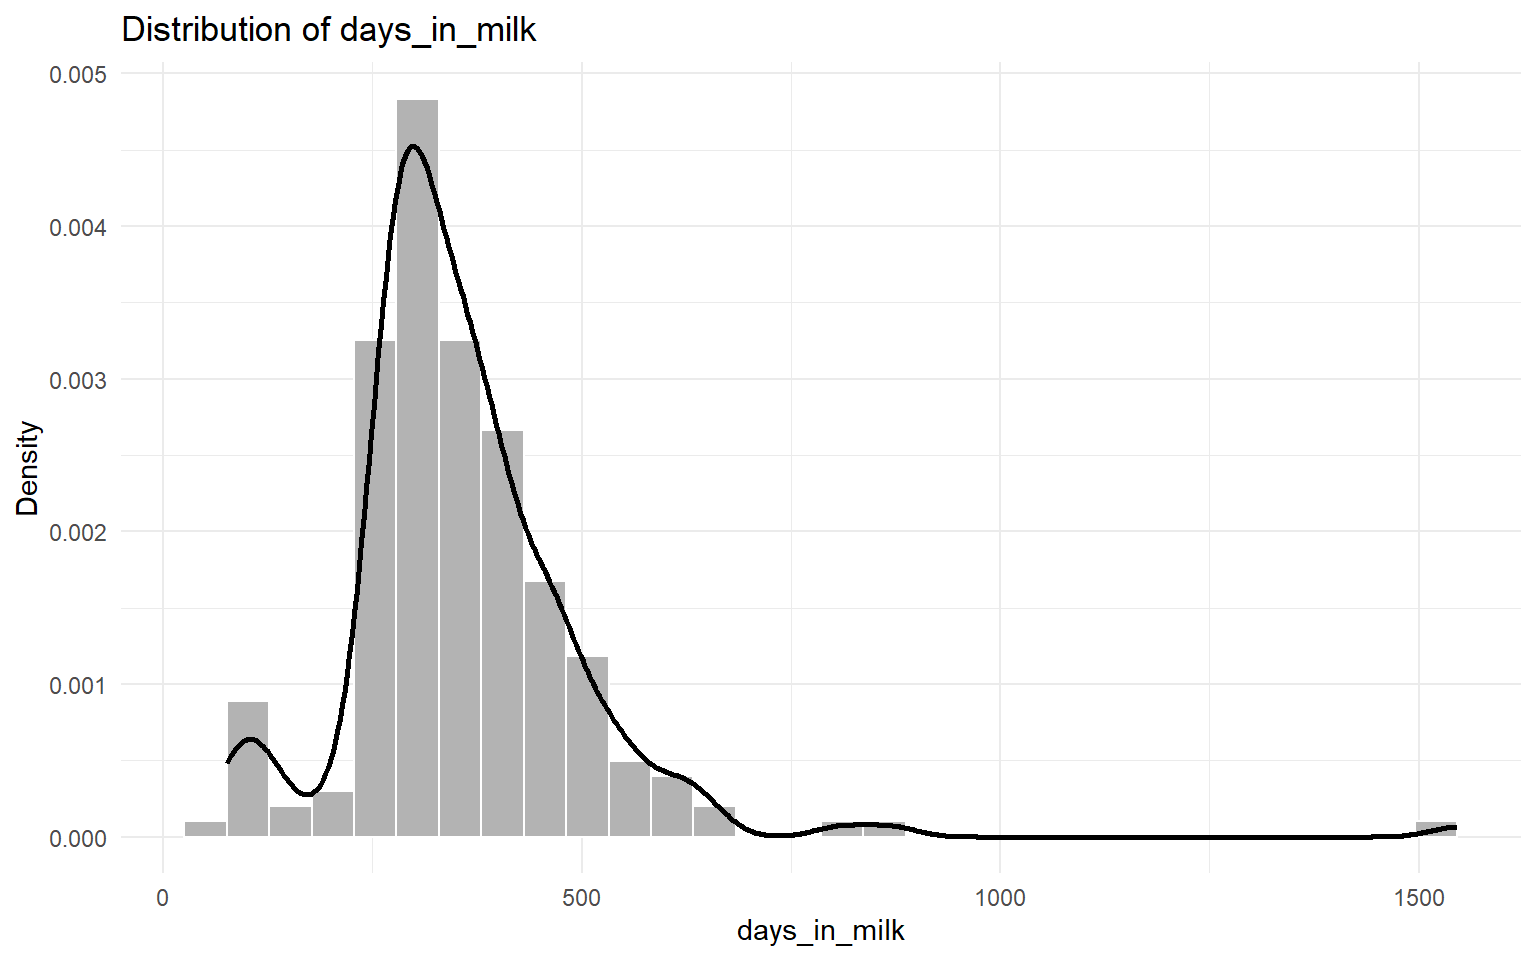
\includegraphics[keepaspectratio]{check_genotype_data_files/figure-latex/unnamed-chunk-2-1.pdf}}
\pandocbounded{\includegraphics[keepaspectratio]{check_genotype_data_files/figure-latex/unnamed-chunk-2-2.pdf}}
\pandocbounded{\includegraphics[keepaspectratio]{check_genotype_data_files/figure-latex/unnamed-chunk-2-3.pdf}}
\pandocbounded{\includegraphics[keepaspectratio]{check_genotype_data_files/figure-latex/unnamed-chunk-2-4.pdf}}

\begin{verbatim}
## [holstein] Total SNPs: 47,576; failing any filter: 5,962 (12.53%)
\end{verbatim}

\begin{verbatim}
## === Processing breed: jersey ===
## smiss head:
\end{verbatim}

\begin{verbatim}
## # A tibble: 6 x 5
##     FID   IID MISSING_CT OBS_CT   F_MISS
##   <dbl> <dbl>      <dbl>  <dbl>    <dbl>
## 1   201  4273         56  47576 0.00118 
## 2   202  4284         69  47576 0.00145 
## 3   203  4289         54  47576 0.00114 
## 4   204  4230         52  47576 0.00109 
## 5   205  4292         27  47576 0.000568
## 6   206  4236         32  47576 0.000673
\end{verbatim}

\begin{verbatim}
## vmiss head:
\end{verbatim}

\begin{verbatim}
## # A tibble: 6 x 5
##   CHROM ID                              MISSING_CT OBS_CT F_MISS
##   <chr> <chr>                                <dbl>  <dbl>  <dbl>
## 1 1     Hapmap43437-BTA-101873                   0     96      0
## 2 1     ARS-BFGL-NGS-16466                       0     96      0
## 3 1     ARS-BFGL-NGS-105096                      0     96      0
## 4 1     Hapmap34944-BES1_Contig627_1906          0     96      0
## 5 1     ARS-BFGL-NGS-98142                       0     96      0
## 6 1     Hapmap53946-rs29015852                   0     96      0
\end{verbatim}

\begin{verbatim}
## hardy head:
\end{verbatim}

\begin{verbatim}
## # A tibble: 6 x 11
##   CHROM ID               A1    AX    HOM_A1_CT HET_A1_CT TWO_AX_CT `O(HET_A1)`
##   <dbl> <chr>            <chr> <chr>     <dbl>     <dbl>     <dbl>       <dbl>
## 1     1 Hapmap43437-BTA~ G     A            78        18         0       0.188
## 2     1 ARS-BFGL-NGS-16~ G     A            70        26         0       0.271
## 3     1 ARS-BFGL-NGS-10~ G     A            16        57        23       0.594
## 4     1 Hapmap34944-BES~ C     A            10        52        34       0.542
## 5     1 ARS-BFGL-NGS-98~ G     A            49        34        13       0.354
## 6     1 Hapmap53946-rs2~ G     A            46        45         5       0.469
## # i 3 more variables: `E(HET_A1)` <dbl>, P <dbl>, minuslog10P <dbl>
\end{verbatim}

\begin{verbatim}
## afreq head:
\end{verbatim}

\begin{verbatim}
## # A tibble: 6 x 8
##   CHROM ID            REF   ALT   `PROVISIONAL_REF?` ALT_FREQS OBS_CT MAF_calc
##   <chr> <chr>         <chr> <chr> <chr>                  <dbl>  <dbl>    <dbl>
## 1 1     Hapmap43437-~ G     A     Y                     0.0938    192   0.0938
## 2 1     ARS-BFGL-NGS~ G     A     Y                     0.135     192   0.135 
## 3 1     ARS-BFGL-NGS~ G     A     Y                     0.536     192   0.464 
## 4 1     Hapmap34944-~ C     A     Y                     0.625     192   0.375 
## 5 1     ARS-BFGL-NGS~ G     A     Y                     0.312     192   0.312 
## 6 1     Hapmap53946-~ G     A     Y                     0.286     192   0.286
\end{verbatim}

\pandocbounded{\includegraphics[keepaspectratio]{check_genotype_data_files/figure-latex/unnamed-chunk-2-5.pdf}}
\pandocbounded{\includegraphics[keepaspectratio]{check_genotype_data_files/figure-latex/unnamed-chunk-2-6.pdf}}
\pandocbounded{\includegraphics[keepaspectratio]{check_genotype_data_files/figure-latex/unnamed-chunk-2-7.pdf}}

\begin{verbatim}
## Warning: Removed 3 rows containing non-finite outside the scale range (`stat_bin()`).
## Removed 3 rows containing non-finite outside the scale range (`stat_bin()`).
\end{verbatim}

\pandocbounded{\includegraphics[keepaspectratio]{check_genotype_data_files/figure-latex/unnamed-chunk-2-8.pdf}}

\begin{verbatim}
## [jersey] Total SNPs: 47,576; failing any filter: 12,501 (26.28%)
\end{verbatim}

\subsection{Combined summary}\label{combined-summary}

\begin{Shaded}
\begin{Highlighting}[]
\NormalTok{summary\_all }\OtherTok{\textless{}{-}}\NormalTok{ dplyr}\SpecialCharTok{::}\FunctionTok{bind\_rows}\NormalTok{(summary\_rows)}
\NormalTok{readr}\SpecialCharTok{::}\FunctionTok{write\_csv}\NormalTok{(summary\_all, }\FunctionTok{file.path}\NormalTok{(base\_dir, }\StringTok{"qc\_summary\_by\_breed.csv"}\NormalTok{))}
\end{Highlighting}
\end{Shaded}

\begin{longtable}[t]{lrrrrrrrr}
\toprule
breed & n\_samples & n\_variants & samples\_over\_mind & snps\_over\_geno & snps\_fail\_hwe & snps\_below\_maf\_threshold & snps\_fail\_any\_filter & pct\_fail\_any\\
\midrule
holstein & 200 & 47576 & 0 & 193 & 108 & 5751 & 5962 & 12.532\\
jersey & 96 & 47576 & 0 & 154 & 48 & 12373 & 12501 & 26.276\\
\bottomrule
\end{longtable}

📦 Outputs

Per-breed (in 02\_reports/\textless breed\textgreater/)

Where

Filename(s)

Format

Description

02\_reports/\textless breed\textgreater/figs/

smiss\_hist.png, vmiss\_hist.png, hardy\_hist.png, maf\_hist.png

PNG

Histogram figures: sample/variant missingness, HWE (−log10P), and MAF

02\_reports/\textless breed\textgreater/

bad\_samples\_over\_mind.\textless breed\textgreater.csv
bad\_snps\_over\_geno.\textless breed\textgreater.csv
bad\_snps\_hwe.\textless breed\textgreater.csv
bad\_snps\_low\_maf.\textless breed\textgreater.csv

CSV

Outlier lists by metric (sample missingness, SNP missingness, HWE, MAF)

02\_reports/\textless breed\textgreater/

variant\_qc\_summary.\textless breed\textgreater.csv

CSV

Per-variant summary with flags (fail\_miss, fail\_hwe, fail\_maf,
fail\_any)

02\_reports/\textless breed\textgreater/

qc\_summary\_counts.csv

CSV

Per-breed counts (samples/variants and how many fail each filter)

Combined (across breeds)

📚 All-breeds summary: 02\_reports/qc\_summary\_by\_breed.csv (CSV)

\subsection{Recap by breed}\label{recap-by-breed}

holstein: 200 samples, 47,576 variants; 5,962 variants (12.53\%) flagged
by any filter (miss=193, HWE=108, low MAF=5,751). Outputs in
02\_reports/holstein/.

jersey: 96 samples, 47,576 variants; 12,501 variants (26.28\%) flagged
by any filter (miss=154, HWE=48, low MAF=12,373). Outputs in
02\_reports/jersey/.

\end{document}
